\chapter{Problem Definition and Research Scope}
\label{chapter:objectives-problem}

This chapter defines the research setting of the thesis. Whereas Chapter~\ref{chapter:introduction} introduced the problem motivation and Chapter~\ref{chapter:literature-review} identified the scientific gap, this chapter clarifies the system under study, the decision hierarchy, and the scope of the proposed execution layer. Rather than restating why the topic matters, it specifies the problem being addressed, the level at which decisions are made, and the assumptions that bound the analysis.

\section{Research Focus}

The central objective of this thesis is to improve the real-time execution of interval-based rebalancing decisions in a free-floating e-scooter system under stochastic demand. More specifically, it examines how relocation guidance generated by an upstream OR rebalancing model can be implemented more selectively at the trip level as system conditions evolve.

The focus is therefore on execution rather than plan generation. The thesis does not attempt to redesign the upstream planning model itself. Instead, it studies how a downstream decision layer can determine whether a suggested relocation should be activated for a specific trip request under the observed system state. This framing follows directly from the gap identified in the previous chapters: interval-based planning may provide useful global guidance, but its operational value ultimately depends on how that guidance is executed in real time.

\section{System Under Study}

The system considered in this thesis is a free-floating shared e-scooter network defined over a discretized urban service area. In the empirical part of the study, it is instantiated as a Rotterdam shared e-scooter case in which the service area is divided into a set of geo-fenced zones. Each zone can function as both an origin and a destination of user trips. This zonal representation provides the spatial resolution needed for relocation planning and execution decisions while also expressing the system state in a form that is operationally meaningful for both the upstream rebalancing model and the downstream execution layer.

Each zone is associated with a finite capacity, reflecting the fact that vehicle accumulation is physically and operationally constrained. As a result, the system is exposed to two different forms of service loss. A zone may experience shortage when too few serviceable scooters are available for departures, and it may experience congestion when additional arrivals cannot be effectively accommodated. This capacity-aware representation is important because it implies that the operational value of a relocation decision depends not only on where vehicles are needed, but also on whether the receiving zone can still absorb redirected arrivals.

The system state is also battery-dependent. Scooters are not treated as identical units; their serviceability depends on battery condition. At the aggregate level, each zone is characterized by an inventory composition across battery categories, which determines how many vehicles are physically present and how many of them are operationally usable. This distinction is essential because two zones with the same total inventory may offer very different service quality if their battery-state composition differs.

System evolution is driven by event-time trip requests rather than solely by decisions at planning boundaries. Each request is characterized by an origin zone, an intended destination zone, a request time, and trip-related user attributes. Once a request arrives, the system must determine whether it proceeds normally or whether an incentive-based relocation option should be considered. For eligible requests, the execution context may include a relocation suggestion generated by the upstream OR rebalancing model. Such a suggestion links the arriving trip to a candidate alternative destination that is expected to improve future system performance.

Taken together, the system combines four sources of operational complexity: stochastic demand, battery-dependent vehicle availability, finite destination capacity, and uncertain user response to relocation incentives. These characteristics make the execution problem fundamentally state-dependent. A relocation suggestion that is beneficial in one local state may be ineffective or even counterproductive in another. The system definition is therefore more than descriptive; it motivates the need for a trip-level execution mechanism that reacts to realized system conditions rather than relying only on interval-level planning outputs.


\section{Decision Hierarchy}

\begin{figure}[H]
    \centering
    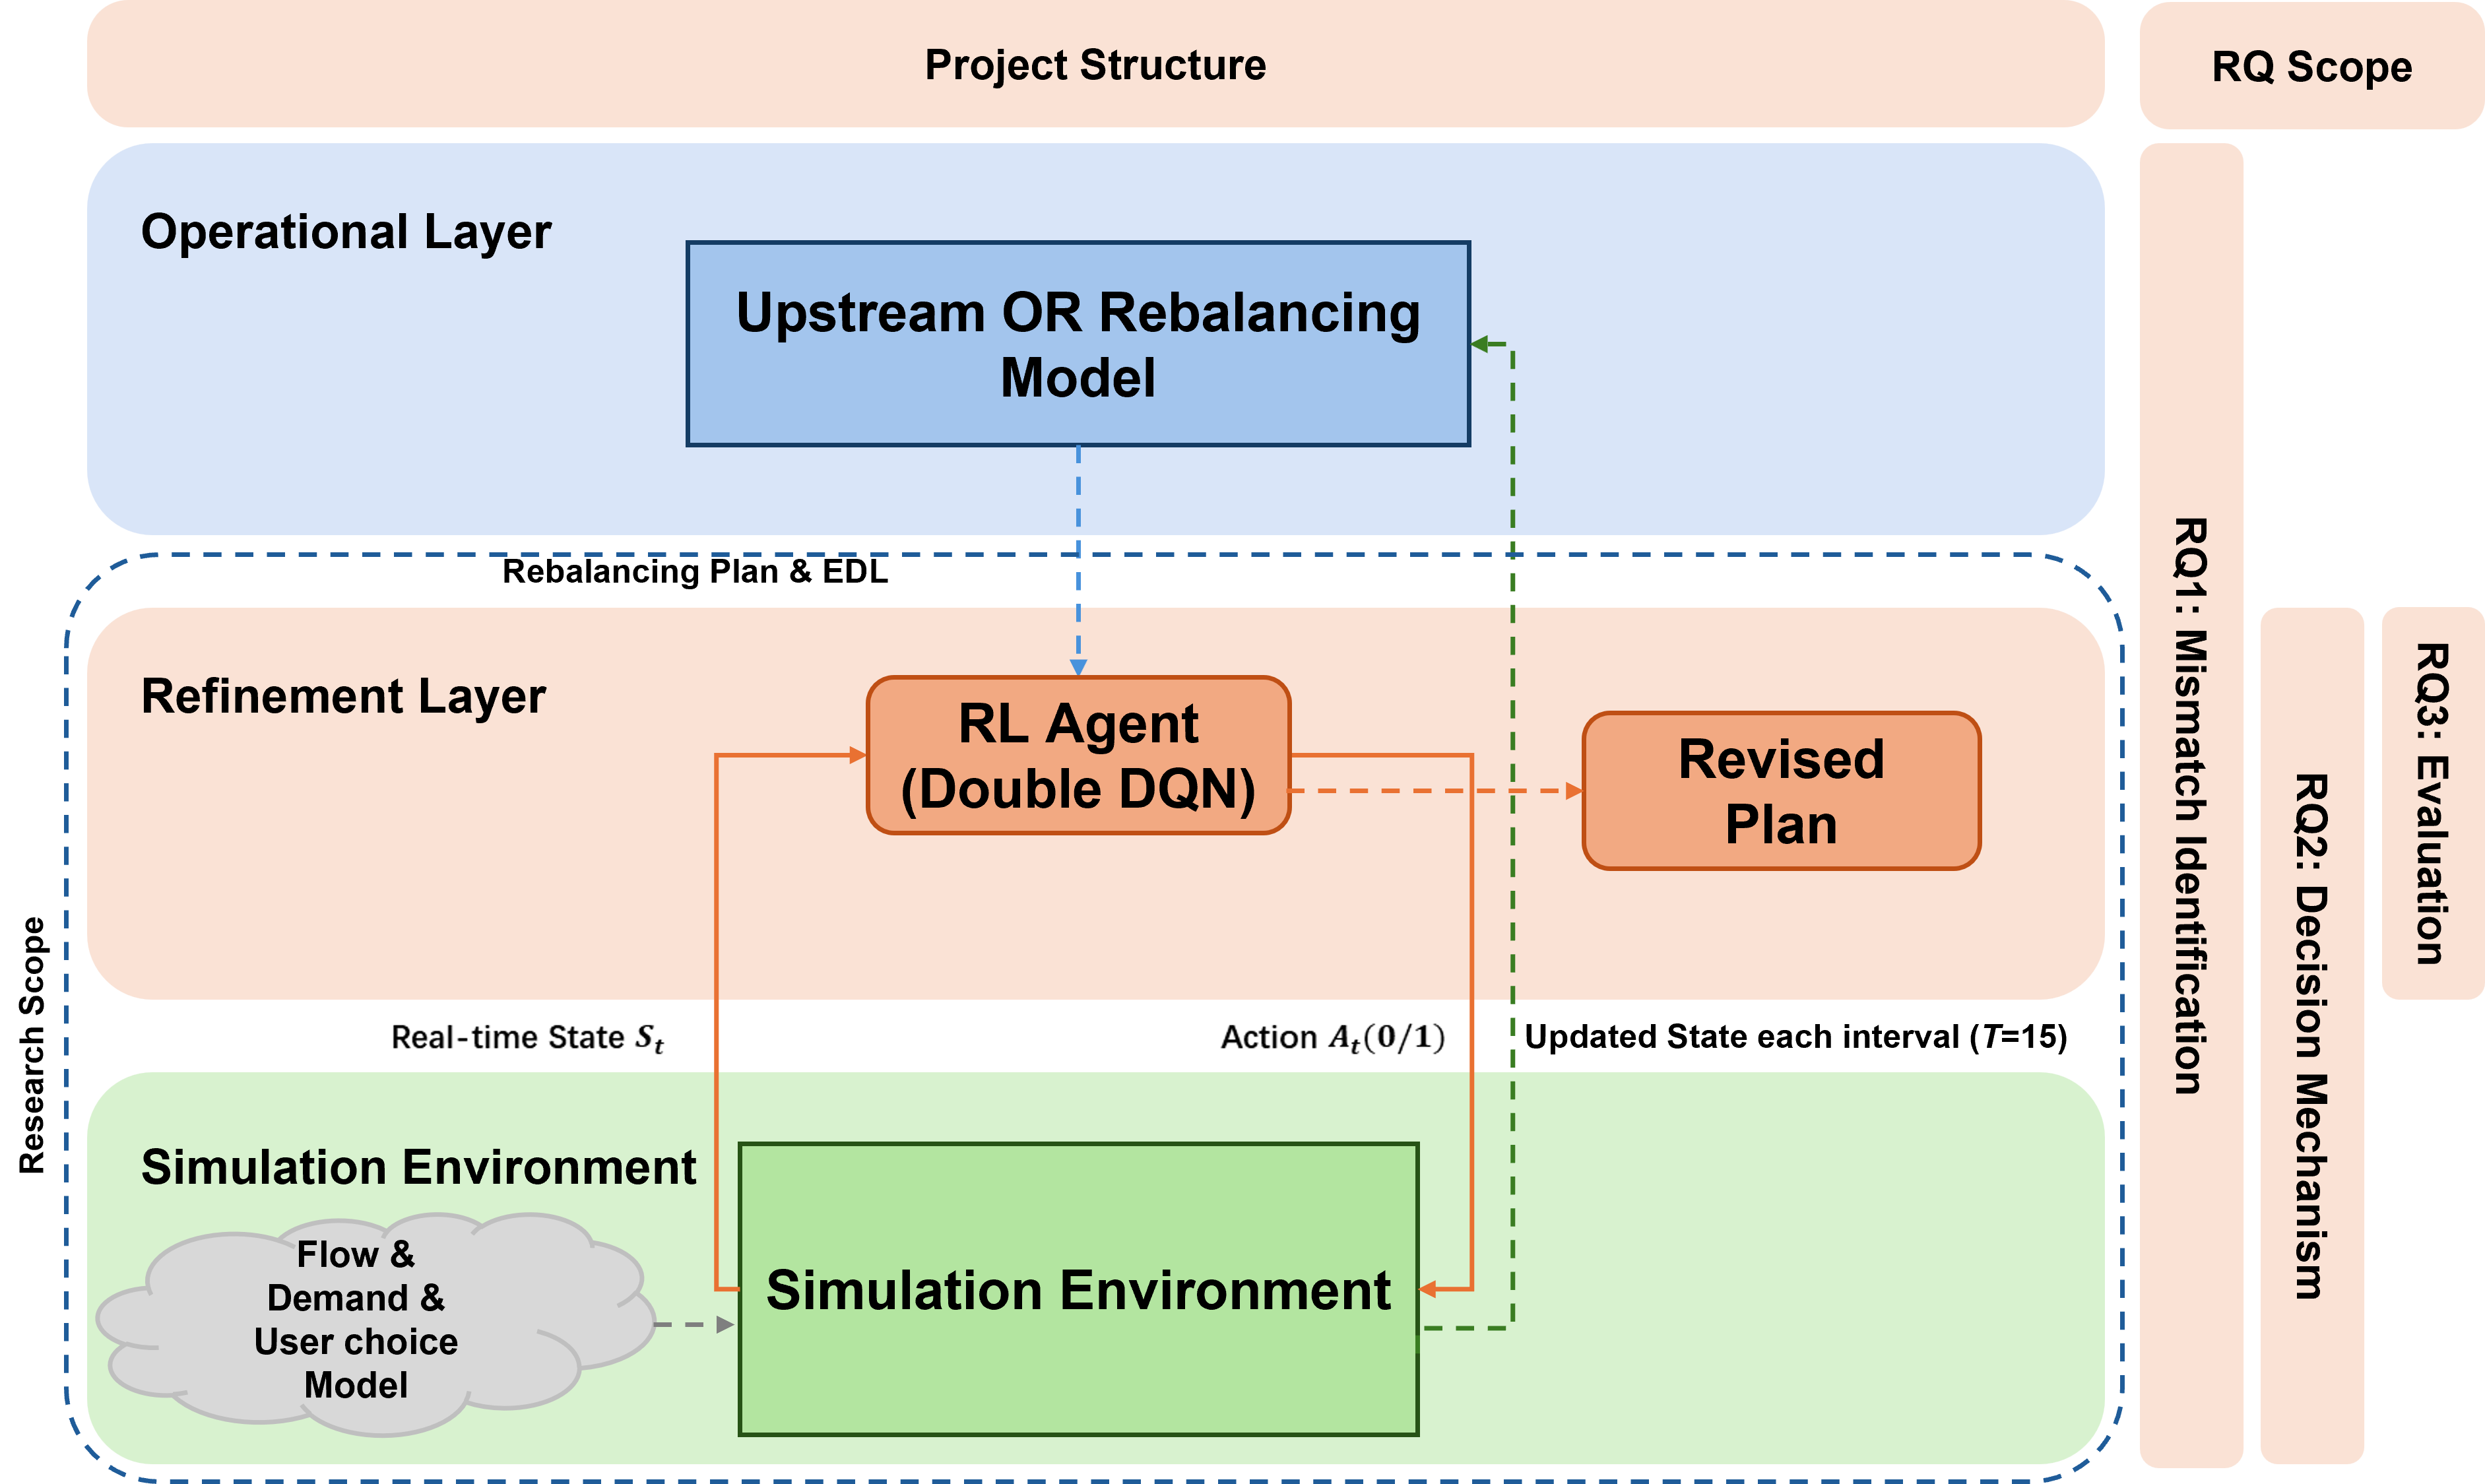
\includegraphics[width=1\textwidth]{figures/figure.png}
    \caption{Layered decision hierarchy and analytical scope of the research questions.}
    \label{fig:decision-hierarchy}
\end{figure}

Figure~\ref{fig:decision-hierarchy} illustrates the layered research structure of the thesis, including the upstream rebalancing model, the trip-level refinement layer, the simulation environment, and the analytical scope of RQ1--RQ3.

The thesis adopts a two-layer decision hierarchy. The upper layer is an interval-based rebalancing model that produces relocation guidance, such as target inventory levels, recommended relocation directions, or candidate relocation trips over a planning horizon. Operating on discretized intervals, this layer provides the global planning logic of the system.

The lower layer is the trip-level execution layer studied in this thesis. Its role is not to recompute the rebalancing plan, but to decide whether guidance from the upper layer should be activated when an eligible trip request arrives. This decision is based on the observed real-time system state and the local execution context. In this way, the upper layer defines relocation intent, while the lower layer determines whether that intent should be implemented for a specific trip.

This separation is central to the scope of the thesis. It keeps the analysis focused on the planning--execution interface rather than expanding into a full redesign of the control architecture. It also makes the research question operationally meaningful: even with a fixed upstream rebalancing model, substantial performance gains may still be achieved through better trip-level execution.

\section{Formal Problem Definition}

The execution problem studied in this thesis is defined at the level of individual eligible trip requests. At each decision epoch, a request arrives in continuous time. For that request, the system observes the current network state, checks whether relocation guidance exists for the request context, and determines whether an incentive should be issued.

The decision input consists of four main elements. First, the observed system state describes zone-level inventory conditions, battery composition, and other operational signals relevant to near-term service performance. Second, the trip request itself provides origin, intended destination, and request timing information. Third, the upstream OR model or rebalancing model may provide a suggested relocation target or indicate that the request belongs to the eligible execution scope. Fourth, uncertainty remains in the form of user acceptance, future realized demand, and evolving resource availability.

Under this setting, the action space is binary: offer or do not offer. If no incentive is offered, the trip proceeds according to its original execution path. If an incentive is offered, the user may either accept the relocation or reject it, and the realized outcome influences the subsequent system state. The objective is to improve service-related outcomes and incentive efficiency by making better execution decisions at the moment of request arrival.

This problem formulation makes the refinement layer event-driven, state-dependent, and stochastic. Decisions are triggered by trip arrivals, their desirability depends on the local system state, and both demand realization and user response remain uncertain even after a decision has been made.

\section{Scope and Delimitations}

The scope of the thesis is intentionally narrow. The study focuses on trip-level selective execution of relocation guidance in a shared e-scooter setting. The upstream OR model or rebalancing model is treated as an external planning input rather than as an object of redesign. Likewise, the incentive mechanism is studied in a simplified binary form, where the operational question is whether to trigger an offer rather than how to optimize a continuous price signal.

Several elements are therefore outside the scope of this thesis. The study does not redesign the upstream OR model, examine continuous incentive pricing, or formulate a full joint optimization of planning and execution. It also does not attempt to solve a wider operational fleet-management problem involving all relocation levers simultaneously, such as truck routing, battery swapping logistics, and joint multi-operator dispatching. The goal is narrower and more precise: to isolate the value of a trip-level execution layer under uncertainty.

This restricted scope keeps the action space interpretable, allows the planning--execution interface to be studied directly, and makes the resulting framework easier to evaluate in simulation. It also aligns with the broader logic of the thesis: the contribution lies in refining execution, not in replacing the entire system architecture.

\section{Mapping of Research Questions to Analysis}

The three research questions introduced in Chapter~\ref{chapter:introduction} map directly onto the analytical structure of the thesis. RQ1 addresses execution mismatch identification by examining how interval-based relocation guidance can diverge from realized trip-level system conditions once stochastic demand, battery-state changes, and local capacity constraints begin to unfold within a planning interval.

RQ2 addresses decision-mechanism design by specifying how the trip-level execution problem should be represented in terms of state, action, uncertainty, and operational objective. This question motivates the formal design of the refinement layer developed in the later methodological chapters.

RQ3 addresses comparative performance evaluation by defining how the proposed execution mechanism will be compared against baseline policies and how resulting changes in service-related outcomes and incentive efficiency will be measured. This evaluation logic supports the empirical chapters that follow.

By structuring the research questions in this way, the thesis maintains a clear progression: identify the operational mismatch, define the trip-level decision problem, and then evaluate whether the proposed mechanism improves execution outcomes.

\section{Chapter Summary}

This chapter has defined the research setting of the thesis in formal terms. It has clarified that the study concerns a free-floating e-scooter system with stochastic demand, battery-dependent vehicle availability, and externally provided relocation guidance. It has also distinguished the upstream OR model or rebalancing model from the downstream trip-level execution layer and specified the scope of the thesis as one of selective execution rather than full planning redesign. With this problem definition in place, the next chapter introduces the methodological framework used to study the proposed execution mechanism.
